%%%%%%%%%%%%%%%%%%%%%%%%%%%%%%%%%%%%%%%%%%%%%%%%%%%%%%%%
%%%%                                              %%%%%%
%%%%  Author: Peter Wilson                        %%%%%%
%%%%                                              %%%%%%
%%%%     Extension of DSG element technology                  %%%%%%
%%%%                                              %%%%%%
%%%%%%%%%%%%%%%%%%%%%%%%%%%%%%%%%%%%%%%%%%%%%%%%%%%%%%%%


%fref generates automatically the respective abreviation/word in the text for the reference. You just have to define a label starting with the respective keyword.
%english: chap, sec, fig, eq, app
%deutsch: chap/kap, abs, abb, gl, anh
%see http://ctan.space-pro.be/tex-archive/macros/latex/contrib/fancyref/fancyref.pdf for more \section

%\onehalfspacing
%\setlength{\belowcaptionskip}{-17pt}

\chapter[Extension of DSG linear triangle element technology]{Extension of DSG \\ linear triangle element \\ technology}
\label{chap:chapter_dsg_extension}

\renewcommand{\Thema}{Extension of DSG linear triangle element technology}

\lettrine[lines=2]{A}{lthough} the DSG element technology drastically enhances the performance of the basic constant strain triangle (Basic-T3) formulation in a very computationally efficient package, the drawback of nodal numbering dependency in coarse linear triangular meshes has tempted academics since it's original publication to extend the elegant underlying discrete shear gap concept into a formulation invariant of nodal ordering. This chapter concerns itself with: one such formulation under development with promising initial results, another approach successfully published and gaining traction and illuminating the severity of the DSG nodal numbering sensitivity in order to ascertain whether remedies are actually worthwhile in practical scenarios.

\section{DSGc3 approach}
The DSGc3 approach is a method under development lead by Prof. Bletzinger at TUM's chair of structural engineering aimed at addressing the aforementioned nodal numbering dependency of Bletzinger's original DSG formulation. In it's current stage, the DSGc3 approach offers a successful proof of concept in the form of a parametric unit triangle formulation, with the next stage in development being the extension into arbitrary Cartesian triangles. 

\subsection{DSGc3 unit triangle parametric formulation}
Consider the following parametric unit triangle with nodal coordinates $(\xi_i,\eta_i)$ = $(0,0),\ (1,0),\ (0,1)$ as per the figure below:

\begin{figure}[H]
	\centering
	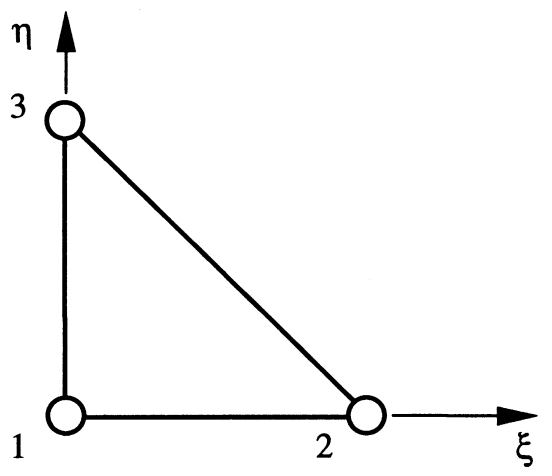
\includegraphics[width=8cm]{images/parametric_unit_triangle.png}
	\caption{Parametric unit triangle \cite{Ble00}}
	\label{fig:parametric_unit_triangle}
\end{figure}

Three transverse displacement fields are set across the triangle: a Kirchhoff-Love field $w_{KL}$, a displacement field due to Reissner-Mindlin shear $w_{RM \gamma}$ and a moderator field $w_{MOD}$ which has the utility of interacting with both preceding fields thereby rendering the element free of locking effects. The form of the three fields are:

\begin{equation} 
w_{KL} = a_1 + \xi a_2 + \eta a_3 + \xi^2 a_4 + 0.5(a_5 + a_6)\xi \eta + \eta^2 a_7
\label{eqDSGc3_1}\ ,
\end{equation}
\begin{equation} 
w_{RM \gamma} = \xi a_8 + \eta a_9
\label{eqDSGc3_2}
\end{equation}
and
\begin{equation} 
w_{MOD} = 0.5(a_5 - a_6)\xi \eta
\label{eqDSGc3_3}\ .
\end{equation}

The coefficients $a_1$ through $a_9$ are ansatz coefficients as yet unknown corresponding to one or more triangle DOFs each.

The interaction between the moderator field and the Kirchhoff-Love fields is introduced along parametric axes as

\begin{equation} 
w_{KL \xi} = w_{KL} + w_{MOD} = a_1 + \xi a_2 + \eta a_3 + \xi^2 a_4 +a_5 \xi \eta + \eta^2 a_7
\label{eqDSGc3_4}
\end{equation}
and
\begin{equation} 
w_{KL \eta} = w_{KL} - w_{MOD} = a_1 + \xi a_2 + \eta a_3 + \xi^2 a_4 +a_6 \xi \eta + \eta^2 a_7
\label{eqDSGc3_5}\ .
\end{equation}

According to it's definition, differentiating the modified Kirchhoff-Love displacement field yields a pure rotation field:

\begin{equation} 
\beta_{KL \xi} = \frac{\partial w_{KL \xi}}{\partial \xi}  = a_2 + 2 \xi a_4 +a_5 \eta
\label{eqDSGc3_8}
\end{equation}
and
\begin{equation} 
\beta_{KL \eta} = \frac{\partial w_{KL \eta}}{\partial \eta}  =a_3 +a_6 \xi + 2 \eta a_7
\label{eqDSGc3_9}
\end{equation}

A displacement gap field can be recovered by identifying the difference between the Reissner-Mindlin shear-displacement and Kirchhoff-Love displacement fields:
\begin{equation} 
\Delta_w = w_{RM\gamma} - w_{KL}  =-a_1 - a_2\xi - a3\eta - a_4\xi^2 - a_7\eta^2 + a_8\xi + a_9\eta - 0.5\eta\xi(a_5 + a_6)
\label{eqDSGc3_10}\ .
\end{equation}

Until now the fields have been written in general terms of unknown ansatz coefficients. The fields can be congealed by considering 9 boundary conditions, sufficient to set-up 9 equations and solve the 9 unknowns.

The first three equations constrain the displacement gap field to fulfil discrete nodal transverse displacements:

\begin{equation} 
bc1 = \Delta_w(0,0) = w_1 = -a_1
\label{eqDSGc3_11}\ ,
\end{equation}
\begin{equation} 
bc2 = \Delta_w(1,0) = w_2 = -a_1 -a_2 -a_4 + a_8
\label{eqDSGc3_12}\ ,
\end{equation}
and
\begin{equation} 
bc3 = \Delta_w(0,1) = w_3 = -a_1 -a_3 -a_7 + a_9
\label{eqDSGc3_13}\ .
\end{equation}

The remaining six impose rotation conditions on the nodal extremities of the modified Kirchhoff-Love fields, shaping both it and the introduced moderator field:

\begin{equation} 
bc4 = \beta_{KL \xi}(0,0) = \beta_{\xi 1} = a_2
\label{eqDSGc3_14}\ ,
\end{equation}
\begin{equation} 
bc5 = \beta_{KL \xi}(1,0) = \beta_{\xi 2} = a_2 + 2a_4
\label{eqDSGc3_15}\ ,
\end{equation}
\begin{equation} 
bc6 = \beta_{KL \xi}(0,1) = \beta_{\xi 3} = a_2 + a_5
\label{eqDSGc3_16}\ ,
\end{equation}

\begin{equation} 
bc7 = \beta_{KL \eta}(0,0) = \beta_{\eta 1} = a_3
\label{eqDSGc3_17}\ ,
\end{equation}
\begin{equation} 
bc8 = \beta_{KL \eta}(1,0) = \beta_{\eta 2} = a_3 + a_6
\label{eqDSGc3_18}\ ,
\end{equation}
and
\begin{equation} 
bc9 = \beta_{KL \eta}(0,1) = \beta_{\eta 3} = a_3 + 2a_7
\label{eqDSGc3_19}\ .
\end{equation}

Solving the above system of equations yields the following ansatz coefficients:

\begin{equation} 
\begin{pmatrix}
a_1 \\
a_2 \\
a_3 \\
a_4 \\
a_5 \\
a_6 \\
a_7 \\
a_8 \\
a_9
\end{pmatrix}
=
\begin{pmatrix}
-w_1 \\
\beta_{\xi 1} \\
\beta_{\eta 1} \\
0.5(\beta_{\xi 2} - \beta_{\xi 1}) \\
\beta_{\xi 3} - \beta_{\xi 1} \\
\beta_{\eta 2} - \beta_{\eta 1} \\
0.5(\beta_{\eta 3} - \beta_{\eta 1}) \\
w_2 - w_1 + 0.5(\beta_{\xi 1} + \beta_{\xi 2}) \\
w_3 - w_1 + 0.5(\beta_{\eta 1} + \beta_{\eta 3}) 
\end{pmatrix}
\label{eqDSGc3_20}\ .
\end{equation}

For completeness, the Reissner-Mindlin shear-displacement and moderator fields are re-written with the ansatz results substituted:

\begin{equation} 
w_{RM \gamma} = \eta(0.5 \beta_{\eta 1} + 0.5\beta_{\eta 3} - w_1 + w_3) + \xi(0.5\beta_{\xi 1} + 0.5\beta_{\xi 2} - w_1 + w_2)
\label{eqDSGc3_21}\ ,
\end{equation}
and
\begin{equation} 
w_{MOD} = \eta\xi(-0.5\beta_{\xi 1}1 + 0.5\beta_{\xi 3} + 0.5\beta_{\eta 1} - 0.5\beta_{\eta 2})
\label{eqDSGc3_22}\ .
\end{equation}

Indeed, the resulting Reissner-Mindlin shear-displacement field above is similar to the DSG field in the original DSG formulation only without skewed geometry interactions accounted for.

As the moderator field was introduced into the Kirchhoff-Love field previously, so can it be introduced into the Reissner-Mindlin shear-displacement field as:

\begin{equation} 
w_{RM \gamma \xi} = w_{RM \gamma} + w_{MOD} 
\label{eqDSGc3_6}
\end{equation}
and
\begin{equation} 
w_{RM \gamma \eta} = w_{RM \gamma} - w_{MOD} 
\label{eqDSGc3_7}\ .
\end{equation}

Similar to the original DSG formulation, the shear deformation field can be precipitated from the modified Reissner-Mindlin shear-displacement field via differentiation, yielding:

\begin{equation} 
\gamma_{RM \gamma \xi} = \frac{\partial w_{RM \gamma \xi}}{\partial \xi}  = 0.5\beta_{\xi 1} + 0.5\beta_{\xi 2} - w_1 + w_2 + \eta(-0.5\beta_{\xi 1} + 0.5\beta_{\xi 3} + 0.5\beta_{\eta 1} - 0.5\beta_{\eta 2})
\label{eqDSGc3_23}
\end{equation} 
and
\begin{equation} 
\gamma_{RM \gamma \eta} = \frac{\partial w_{RM \gamma \eta}}{\partial \eta}  = 0.5\beta_{\xi 1} + 0.5\beta_{\xi 3} - w_1 + w_3 - \xi(-0.5\beta_{\xi 1} + 0.5\beta_{\xi 3} + 0.5\beta_{\xi 1} - 0.5\beta_{\xi 3})
\label{eqDSGc3_25}\ .
\end{equation}

The entries of the above fields can ordered in a strain-displacement B matrix relating the shear fields to the triangle plate theory DOFs, resulting in:

\begin{equation} 
\mathbf{B}_\gamma = 
\begin{pmatrix}
-1 & 1 & 0 & 0.5(1 - \eta) & 0.5 & 0.5\eta & 0.5\eta & -0.5\eta & 0 \\
-1 & 0 & 1 & 0.5\xi & 0 & -0.5\xi & 0.5(1-\xi) & 0.5\xi & 0.5
\end{pmatrix}
\label{eqDSGc3_26}\ .
\end{equation}

\subsection{DSGc3 example}
In order to illustrate the locking-free performance of the DSGc3 proof of concept formulation, a Python implementation of the element solving prescribed displacements is considered. As per the formulation under development, a unit triangle of thickness $h = 0.005$ is considered with isotropic material properties $E = 1000,\ \nu=0.0$ subject to no external influence except the following prescribed displacements: $w_1 = w_3 = 0.5,\ w_2 = \beta_{\xi 1} = \beta_{\eta 1} = 1.0$ and $\beta_{\xi 3} = 1.5$. Thus the DOFs $\beta_{\xi 2},\ \beta_{\eta 2}$ and $\beta_{\eta 3}$ form the problem unknowns. The results of the analysis determine the following unknown values: $\beta_{\xi 2} = -2.0,\ \beta_{\eta 2} = 1.5$ and $\beta_{\eta 3} = -1.0$. Of more interest, however, is the visual representation of the underlying formulation fields, with the various displacement fields fulfilling the solution presented below:

\begin{figure}[H]
	\subfloat[Displacement gap field]
	{\label{ref_label2}
		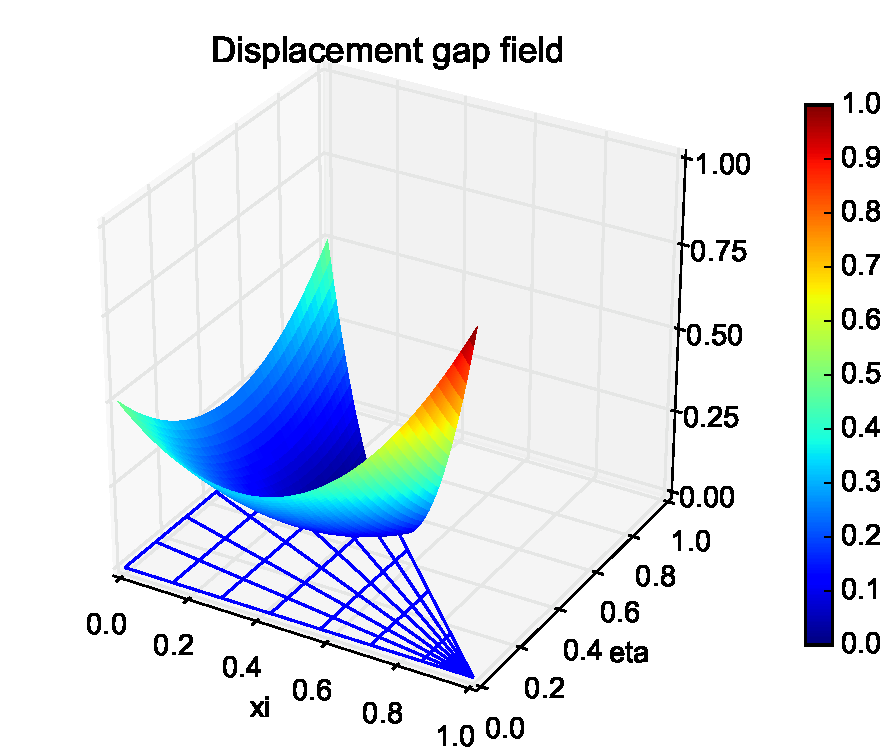
\includegraphics[width=7.3cm]
		{displacement_gap_field.pdf}}
	\subfloat[Displacement gap field - top view]
	{\label{ref_label2}
		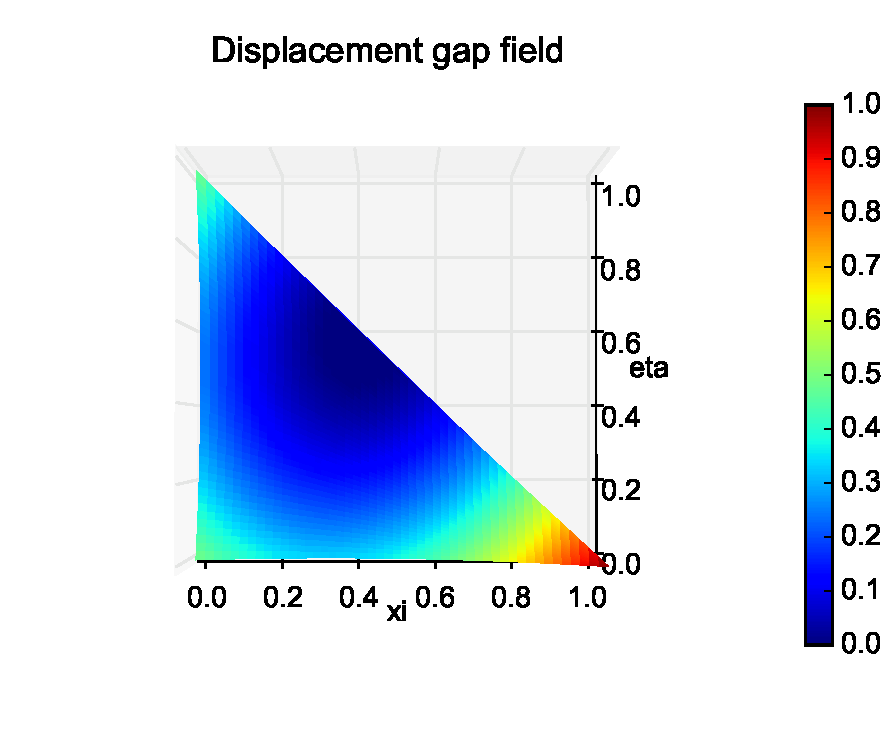
\includegraphics[width=7.3cm]
		{displacement_gap_field_90.pdf}}
	\\
	\subfloat[Kirchhoff displacement field]
	{\label{ref_label2}
		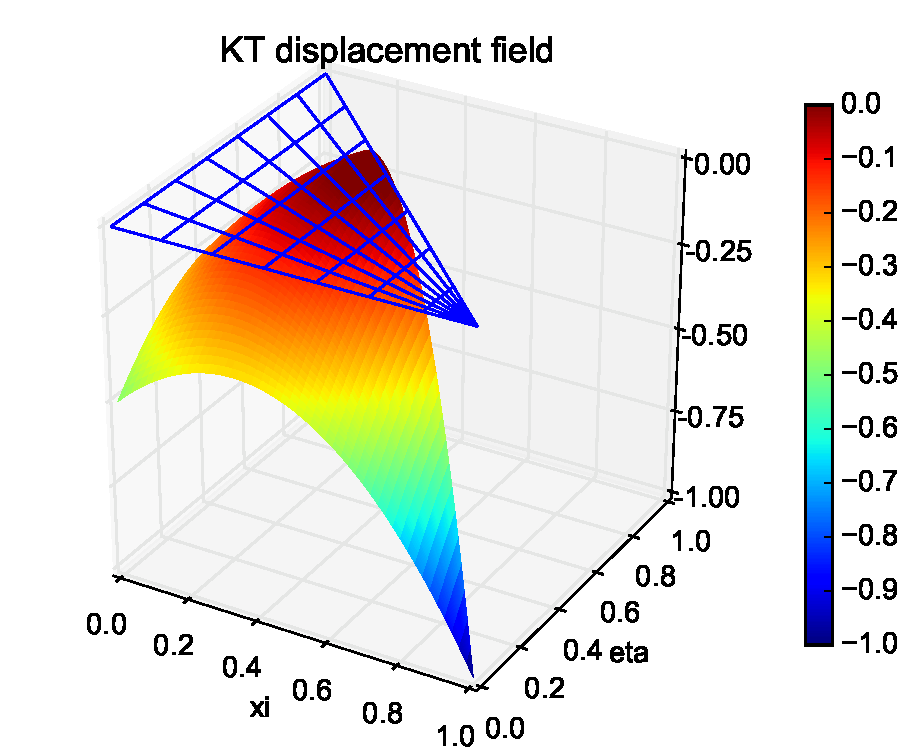
\includegraphics[width=7.3cm]
		{kt_displacement_field.pdf}}
	\subfloat[Kirchhoff displacement field - top view]
	{\label{ref_label2}
		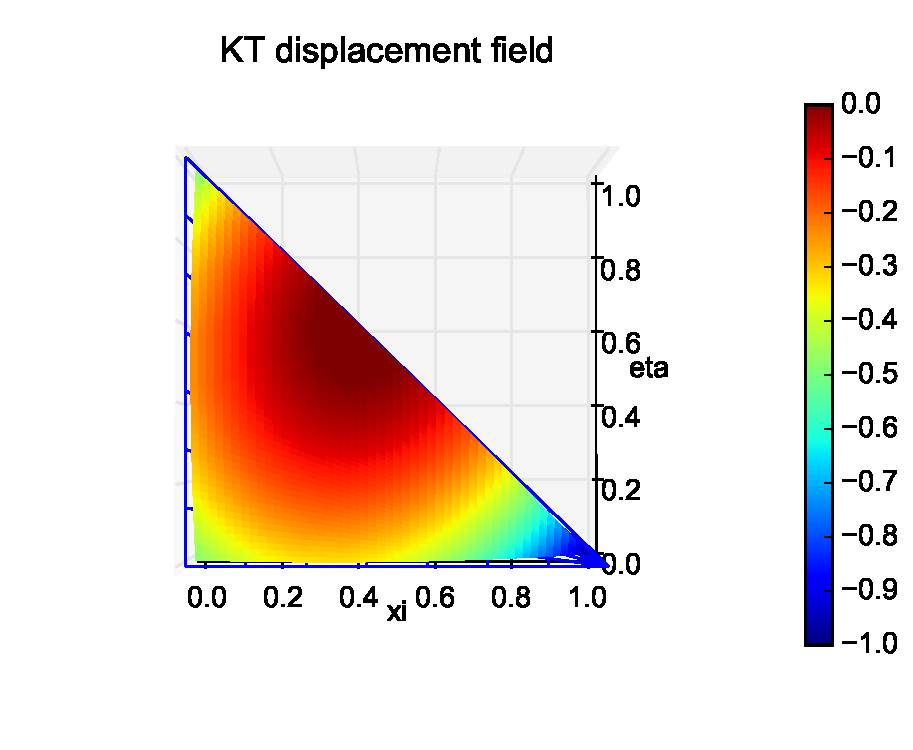
\includegraphics[width=7.3cm]
		{kt_displacement_field_90.pdf}}
	\\
	\subfloat[Reissner-Mindlin shear-displacement field]
	{\label{ref_label2}
		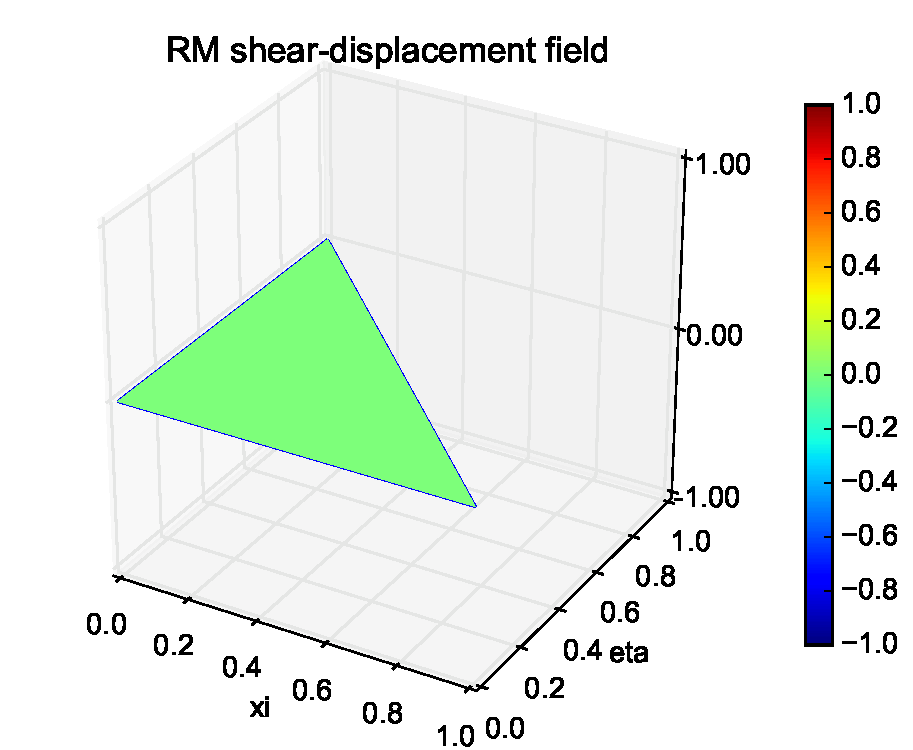
\includegraphics[width=7.3cm]
		{rm_shear_disp_field.pdf}}
	\subfloat[Relationship of aforementioned fields]
	{\label{ref_label2}
		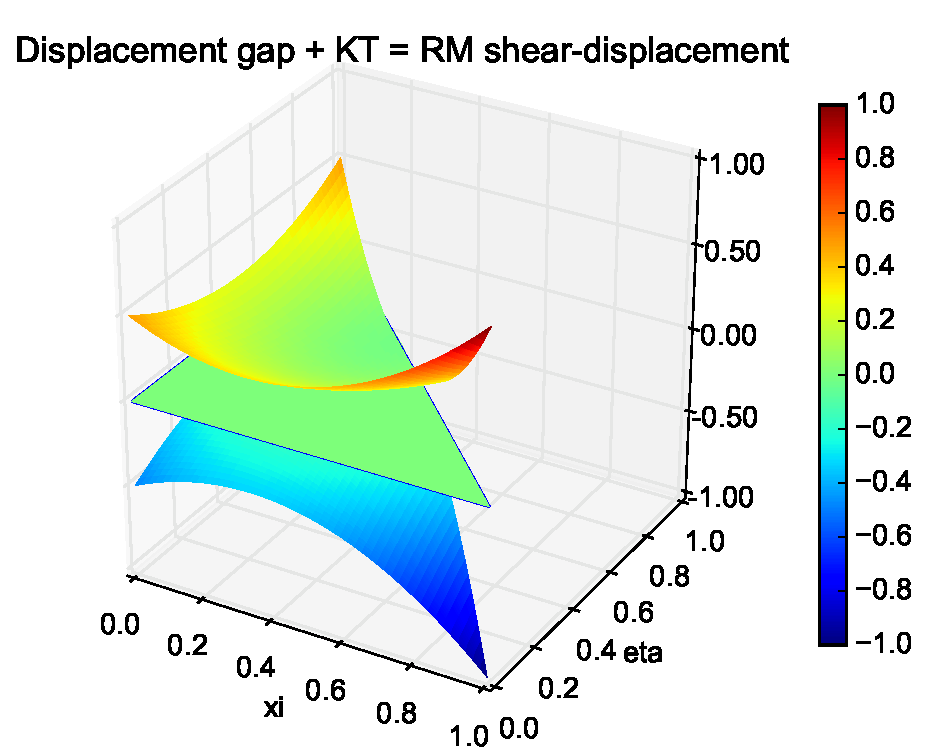
\includegraphics[width=7.3cm]
		{sum.pdf}}
	\caption{\label{csdsgc3_result}DSGc3 example problem displacement field results}
\end{figure}

The displacement gap field in sub-figures (a) and (b) illustrate the fulfilment of nodal transverse displacement as per equations \ref{eqDSGc3_11} through \ref{eqDSGc3_13}, while the Kirchhoff displacement field in sub-figures (c) and (d) fulfils the nodal rotations of equations \ref{eqDSGc3_14} through \ref{eqDSGc3_19}. The locking-free performance of the element is confirmed in (e) with the RM shear-displacement field having a value of zero throughout. Sub-figure (f) highlights the relationship between these three fields, as per equation \ref{eqDSGc3_10}, with the displacement gap and Kirchhoff fields essentially nullifying each other to mitigate locking effects.

The rotation fields of the formulation are presented below:

\begin{figure}[H]
	\subfloat[Rotation xi field]
	{\label{ref_label2}
		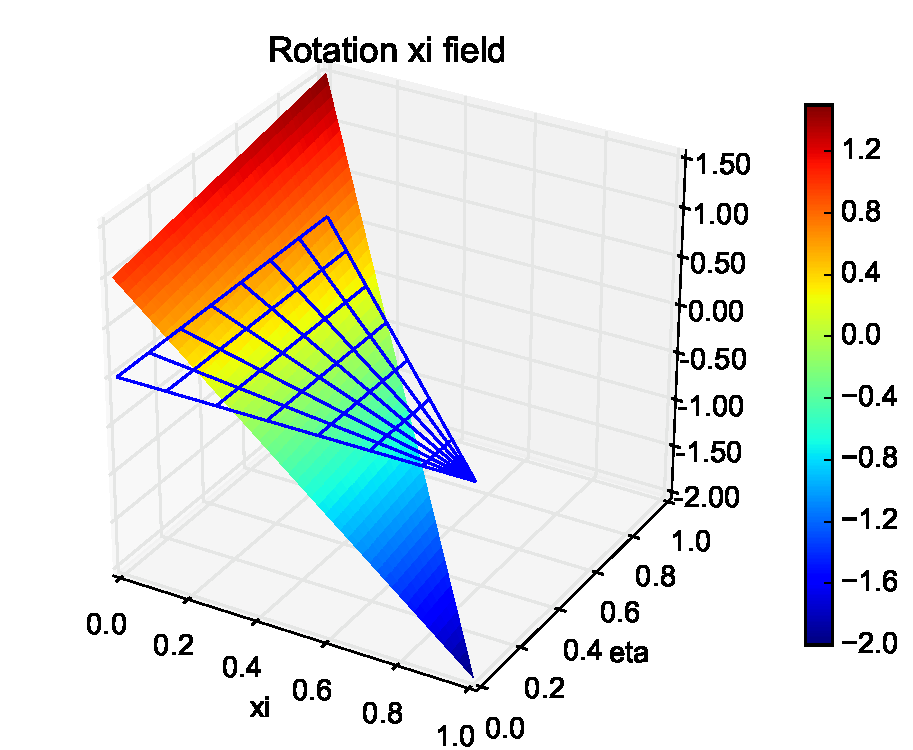
\includegraphics[width=7.3cm]
		{rotation_xi.pdf}}
	\subfloat[Rotation xi field - top view]
	{\label{ref_label2}
		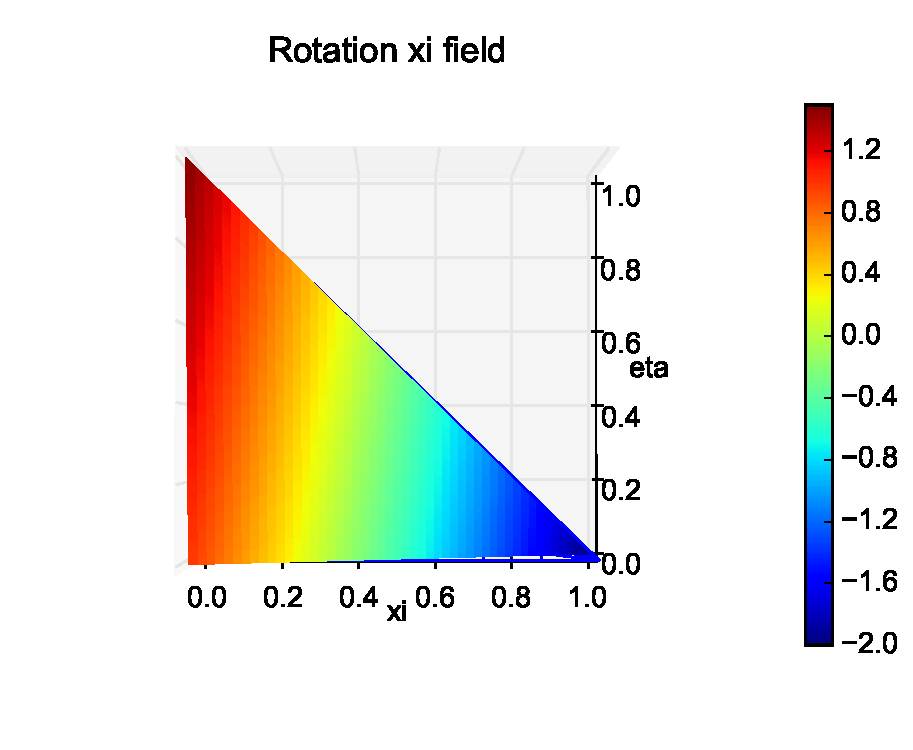
\includegraphics[width=7.3cm]
		{rotation_xi_90.pdf}}
	\\
	\subfloat[Rotation eta field]
	{\label{ref_label2}
		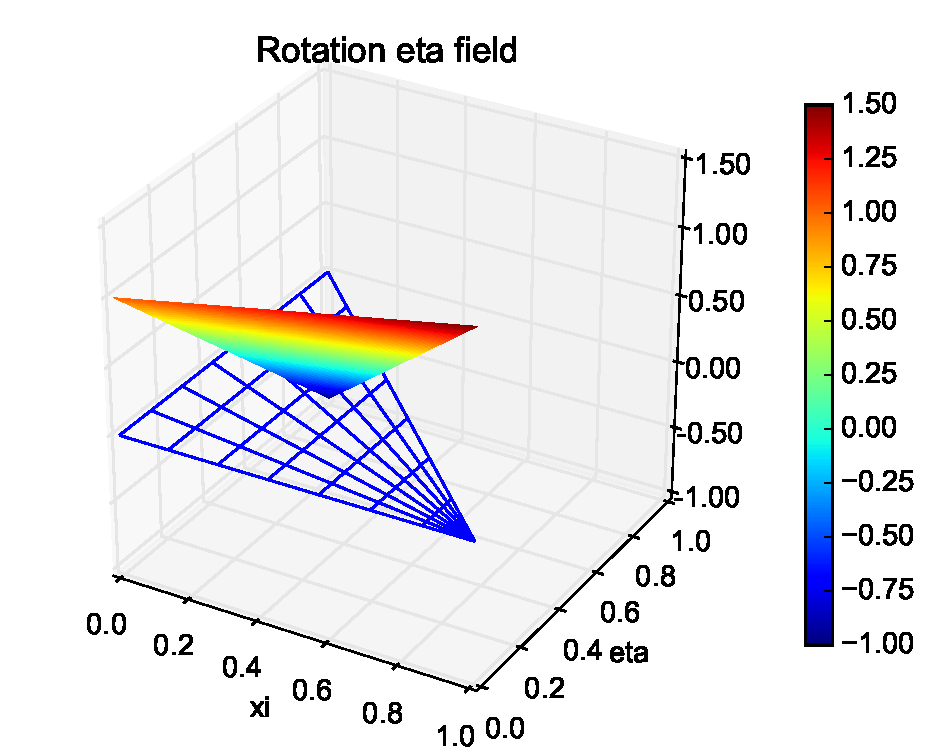
\includegraphics[width=7.3cm]
		{rotation_eta.pdf}}
	\subfloat[Rotation eta field - top view]
	{\label{ref_label2}
		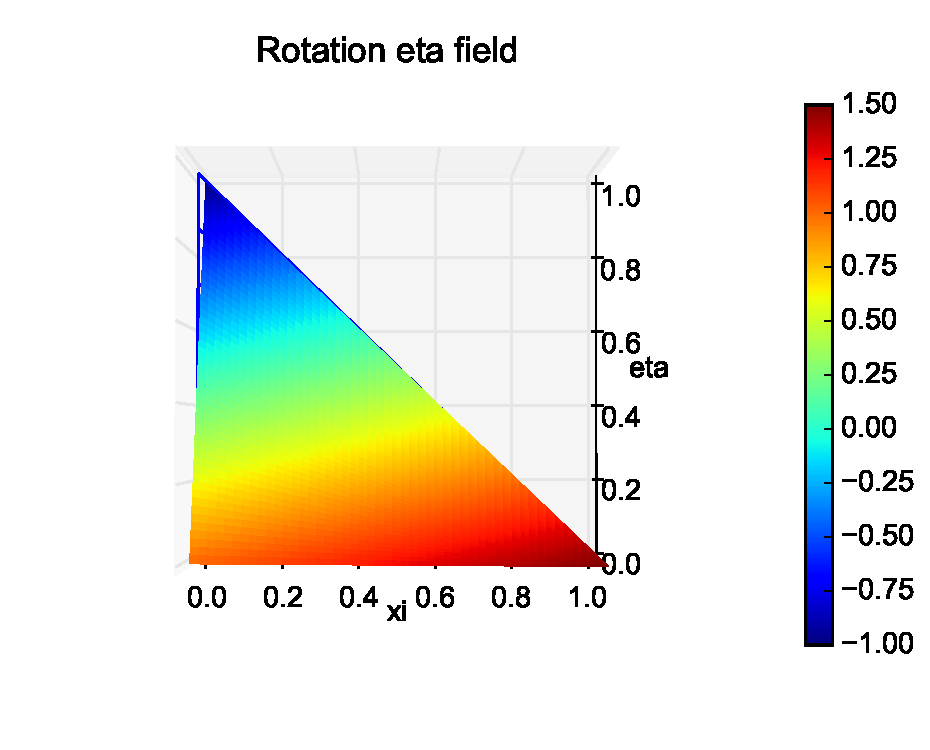
\includegraphics[width=7.3cm]
		{rotation_eta_90.pdf}}
	\caption{\label{csdsgc3_resul1t}DSGc3 example problem rotation field results}
\end{figure}

As per equations \ref{eqDSGc3_8} and \ref{eqDSGc3_9}, both rotation fields exhibit linear interpolation of nodal values, themselves corresponding to the solution values due to the constraints of equations \ref{eqDSGc3_14} though \ref{eqDSGc3_19}.

\subsection{DSGc3 summary}
As an emerging formulation, the DSGc3 offers a promising proof of concept for a locking-free linear triangle element. Further steps to generalise the current unit-triangle parametric formulation to an arbitrarily skewed Cartesian formulation are necessary to effectively use the element in general FEM code, such as Kratos. Thus, given the current state of the DSGc3 formulation, the remaining discussion of extended DSG formulations is limited to the CS-DSG element.

\section{Cell Smoothed DSG approach}
A published and successful approach to remedy the aforementioned nodal numbering dependency is the Cell Smoothed Discrete Shear Gap (CS-DSG) method proposed by Nguyen-Thoi et al. \cite{Ngu13} in 2013. The overarching idea is to split each triangular element into 3 sub-triangles, perform the original DSG formulation on each sub-triangle, then assemble these contributions via an area-averaged approach to recover the behaviour of the meta-triangle. In Reference \cite{Ngu13}, Nguyen-Thoi and his team perform the cell smoothing approach for the membrane, bending and shear B matrices of the original DSG formulation. Since the shear B-matrix is the only component that exhibits nodal ordering dependency, the cell smoothing technique is only applied to the shear B-matrix in this work. The following section illustrates the formulation of the CS-DSG, applied to the shear B-matrix only.

\subsection{CS-DSG formulation}
Crucial to the formulation is the identification of each triangular element's centre point, designated $P_0$, which defines the geometry of the 3 sub-triangles, as per the figure below:

\begin{figure}[H]
	\centering
	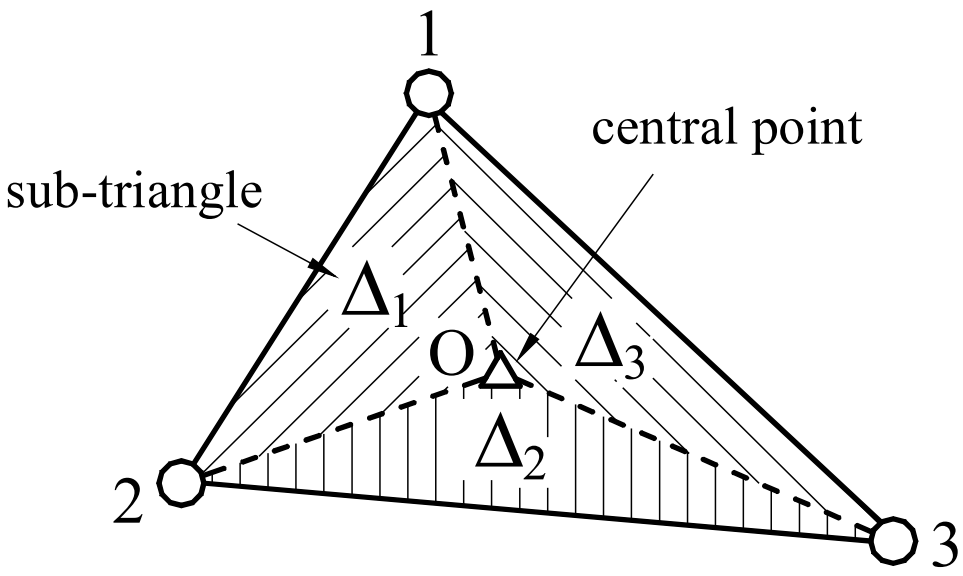
\includegraphics[width=8cm]{images/CSDSG3_subtriangles.png}
	\caption{Division of triangle into 3 sub-triangles about centre point \cite{phung2013static}}
	\label{fig:triangle division}
\end{figure}

The coordinates of the central point are determined from the 3 exterior points as such:

\begin{equation} 
\begin{pmatrix}
x_0 \\
y_0
\end{pmatrix}
=
\frac{1}{3}
\sum_{i=1}^3
\begin{pmatrix}
x_i \\
y_i
\end{pmatrix}
\label{eqCSDSG0}\ .
\end{equation}

As per figure \ref{fig:triangle division}, the displacement vectors for each sub-triangle $\mathbf{u}^{\Delta i}$ are:

\begin{equation} 
\mathbf{u}^{\Delta 1} = 
\begin{pmatrix}
\mathbf{u}_0 \\
\mathbf{u}_1 \\
\mathbf{u}_2
\end{pmatrix}
\ ,
\hspace{10mm}
\mathbf{u}^{\Delta 2} = 
\begin{pmatrix}
\mathbf{u}_0 \\
\mathbf{u}_2 \\
\mathbf{u}_3
\end{pmatrix}
\ ,
\hspace{10mm}
\mathbf{u}^{\Delta 3} = 
\begin{pmatrix}
\mathbf{u}_0 \\
\mathbf{u}_3 \\
\mathbf{u}_1
\end{pmatrix}
\label{eqCSDSG1}\ .
\end{equation}

Critical to the CS-DSG formulation is the relation of $\mathbf{u}_0$ to the exterior nodal displacement vectors which facilitates the central node to be evaporated from the final formulation. According to the geometrical relation, the central point displacement vector can be expressed as:

 \begin{equation} 
\mathbf{u}_0
 =
 \frac{1}{3}
 \sum_{i=1}^3
\mathbf{u}_i
 \label{eqCSDSG2}\ .
 \end{equation}
 
 For each of the sub-triangles $\Delta_i$ the original DSG formulation according to equation \ref{eqt10} is performed, with $x_i,\ y_i$ and $A$ updated to match the nodal positions and area of the current sub-triangle respectively. For illustrative purposes, the first sub-triangle shear B-matrix $\mathbf{B}^{\gamma\Delta 1}$ is written explicitly:
 
\begin{equation}
	\delimitershortfall=0pt
	%\setlength{\dashlinegap}{2pt}
	\mathbf{B}^{\gamma\Delta 1} = 
		\left(\begin{array}{cccccc|cccccc|cccccc}
			0 & 0 & b-c & 0 & A_{\Delta 1} & 0 & 0 & 0 & c & \frac{-bc}{2} & \frac{ac}{2} & 0 & 0 & 0 & -b & \frac{bc}{2} & \frac{-bd}{2} & 0 \\
			0 & 0 & d-a & -A_{\Delta 1} & 0 & 0 & 0 & 0 & -d & \frac{bd}{2} & \frac{-ad}{2} & 0 & 0 & 0 & a & \frac{-ac}{2} & \frac{ad}{2} & 0
		\end{array}
	\right)
	 \label{eqCSDSG3}
\end{equation}

with:

\begin{equation} 
\begin{pmatrix}
a \\
b \\
c \\
d
\end{pmatrix}
=
\begin{pmatrix}
x_{\Delta n2} - x_{\Delta n1} \\
y_{\Delta n2} - y_{\Delta n1} \\
y_{\Delta n3} - y_{\Delta n1} \\
x_{\Delta n3} - x_{\Delta n1} \\
\end{pmatrix}
=
\begin{pmatrix}
x_{1} - x_{0} \\
y_{1} - y_{0} \\
y_{2} - y_{0} \\
x_{2} - x_{0} \\
\end{pmatrix}
\label{eqCSDSG3_0}\ .
\end{equation}

 Furthermore, the shear B-matrix $\mathbf{B}^{\gamma\Delta i}$ for each sub-triangle can be further split into nodal contributions $\mathbf{B}_{\Delta nj}^{\gamma\Delta i}$ corresponding to node $j$ in sub-triangle $i$, continued in the example of the first sub-triangle below:
 
\begin{equation} 
\mathbf{B}_{\Delta n1}^{\gamma\Delta 1}
 =
\begin{pmatrix}
 0 & 0 & b-c & 0 & A_{\Delta 1} & 0 \\
 0 & 0 & d-a & -A_{\Delta 1} & 0 & 0 
\end{pmatrix}
 \label{eqCSDSG4}\ ,
 \end{equation}
 
  \begin{equation} 
\mathbf{B}_{\Delta n2}^{\gamma\Delta 1}
=
\begin{pmatrix}
0 & 0 & c & \frac{-bc}{2} & \frac{ac}{2} & 0 \\
0 & 0 & -d & \frac{bd}{2} & \frac{-ad}{2} & 0
\end{pmatrix}
\label{eqCSDSG5}
\end{equation}
and
  \begin{equation} 
\mathbf{B}_{\Delta n3}^{\gamma\Delta 1}
=
\begin{pmatrix}
0 & 0 & -b & \frac{bc}{2} & \frac{-bd}{2} & 0 \\
0 & 0 & a & \frac{-ac}{2} & \frac{ad}{2} & 0
\end{pmatrix}
\label{eqCSDSG6}
\end{equation}

Thus, the shear strains for sub-triangle 1 can be summarised as:

  \begin{equation} 
\boldsymbol{\gamma}^{\Delta 1} =
\mathbf{B}^{\gamma\Delta 1}
\mathbf{u}^{\Delta 1}
=
\begin{pmatrix}
\mathbf{B}_{\Delta n1}^{\gamma\Delta 1} & \mathbf{B}_{\Delta n2}^{\gamma\Delta 1} & \mathbf{B}_{\Delta n3}^{\gamma\Delta 1}
\end{pmatrix}
\begin{pmatrix}
\mathbf{u}_0 \\
\mathbf{u}_1 \\
\mathbf{u}_2
\end{pmatrix}
\label{eqCSDSG7}\ .
\end{equation}

Recalling equation \ref{eqCSDSG2}, which expresses the central point's displacement vector $\mathbf{u}_0$ in terms of the 3 external node displacement vectors, the shear B-matrix above can similarly be rearranged and expressed in terms of the 3 exterior nodes:

  \begin{equation} 
\boldsymbol{\gamma}^{\Delta 1} =
\mathbf{B}_r^{\gamma\Delta 1}
\mathbf{u}
=
\begin{pmatrix}
\frac{\mathbf{B}_{\Delta n1}^{\gamma\Delta 1}}{3} + \mathbf{B}_{\Delta n2}^{\gamma\Delta 1} & \frac{\mathbf{B}_{\Delta n1}^{\gamma\Delta 1}}{3} + \mathbf{B}_{\Delta n3}^{\gamma\Delta 1} & \frac{\mathbf{B}_{\Delta n1}^{\gamma\Delta 1}}{3}
\end{pmatrix}
\begin{pmatrix}
\mathbf{u}_1 \\
\mathbf{u}_2 \\
\mathbf{u}_3
\end{pmatrix}
\label{eqCSDSG8}\ .
\end{equation}

The above process can be repeated for sub-triangles 2 and 3, yielding the following results:

  \begin{equation} 
\boldsymbol{\gamma}^{\Delta 2} =
\mathbf{B}_r^{\gamma\Delta 2}
\mathbf{u}
=
\begin{pmatrix}
\frac{\mathbf{B}_{\Delta n1}^{\gamma\Delta 2}}{3} &
\frac{\mathbf{B}_{\Delta n1}^{\gamma\Delta 2}}{3} + \mathbf{B}_{\Delta n2}^{\gamma\Delta 2} &
\frac{\mathbf{B}_{\Delta n1}^{\gamma\Delta 2}}{3} + \mathbf{B}_{\Delta n3}^{\gamma\Delta 2} &  
\end{pmatrix}
\begin{pmatrix}
\mathbf{u}_1 \\
\mathbf{u}_2 \\
\mathbf{u}_3
\end{pmatrix}
\label{eqCSDSG9}
\end{equation}
and
  \begin{equation} 
\boldsymbol{\gamma}^{\Delta 3} =
\mathbf{B}_r^{\gamma\Delta 3}
\mathbf{u}
=
\begin{pmatrix}
\frac{\mathbf{B}_{\Delta n1}^{\gamma\Delta 3}}{3} + \mathbf{B}_{\Delta n3}^{\gamma\Delta 3} &
\frac{\mathbf{B}_{\Delta n1}^{\gamma\Delta 3}}{3} &
\frac{\mathbf{B}_{\Delta n1}^{\gamma\Delta 3}}{3} + \mathbf{B}_{\Delta n2}^{\gamma\Delta 3}
\end{pmatrix}
\begin{pmatrix}
\mathbf{u}_1 \\
\mathbf{u}_2 \\
\mathbf{u}_3
\end{pmatrix}
\label{eqCSDSG10}\ .
\end{equation}

With the 3 sub-triangle shear B-matrices expressed in terms of the exterior nodes, they can be recombined via an area-averaged approach to recover the total meta-triangle shear B-matrix $\mathbf{B}^{\gamma}$:

\begin{equation} 
\mathbf{B}^{\gamma}
=
\frac{1}{A_e}
\sum_{i=1}^3
\mathbf{B}_r^{\gamma\Delta i}
A_{\Delta i}
\label{eqCSDSG11}\ .
\end{equation}

\subsection{Invariance of CS-DSG to nodal ordering}
The feature of the CS-DSG formulation is the removal of the original DSG formulation's nodal ordering dependency. The nodal ordering invariance of the CS-DSG formulation is verified with the following example of an equilateral triangle (side lengths $L = 1$, thickness $h = 0.05$) of material properties $E = 1000,\ \nu = 0.29$ fully clamped on it's left side (as per the figure below) subject to a surface pressure of $P_z = -0.01$. The displacement of interest is $u_z$ of point 2 as circled below. 3 tests were performed corresponding to 3 different node ordering arrangements of the triangle: the first being [p1, p3, p2], the second [p3, p2, p1] and the last [p2, p1, p3]. The results of the analysis are presented below.

\begin{figure}[H]
	\subfloat[Nodal ordering sensitivity study setup]
	{\label{ref_label2}
		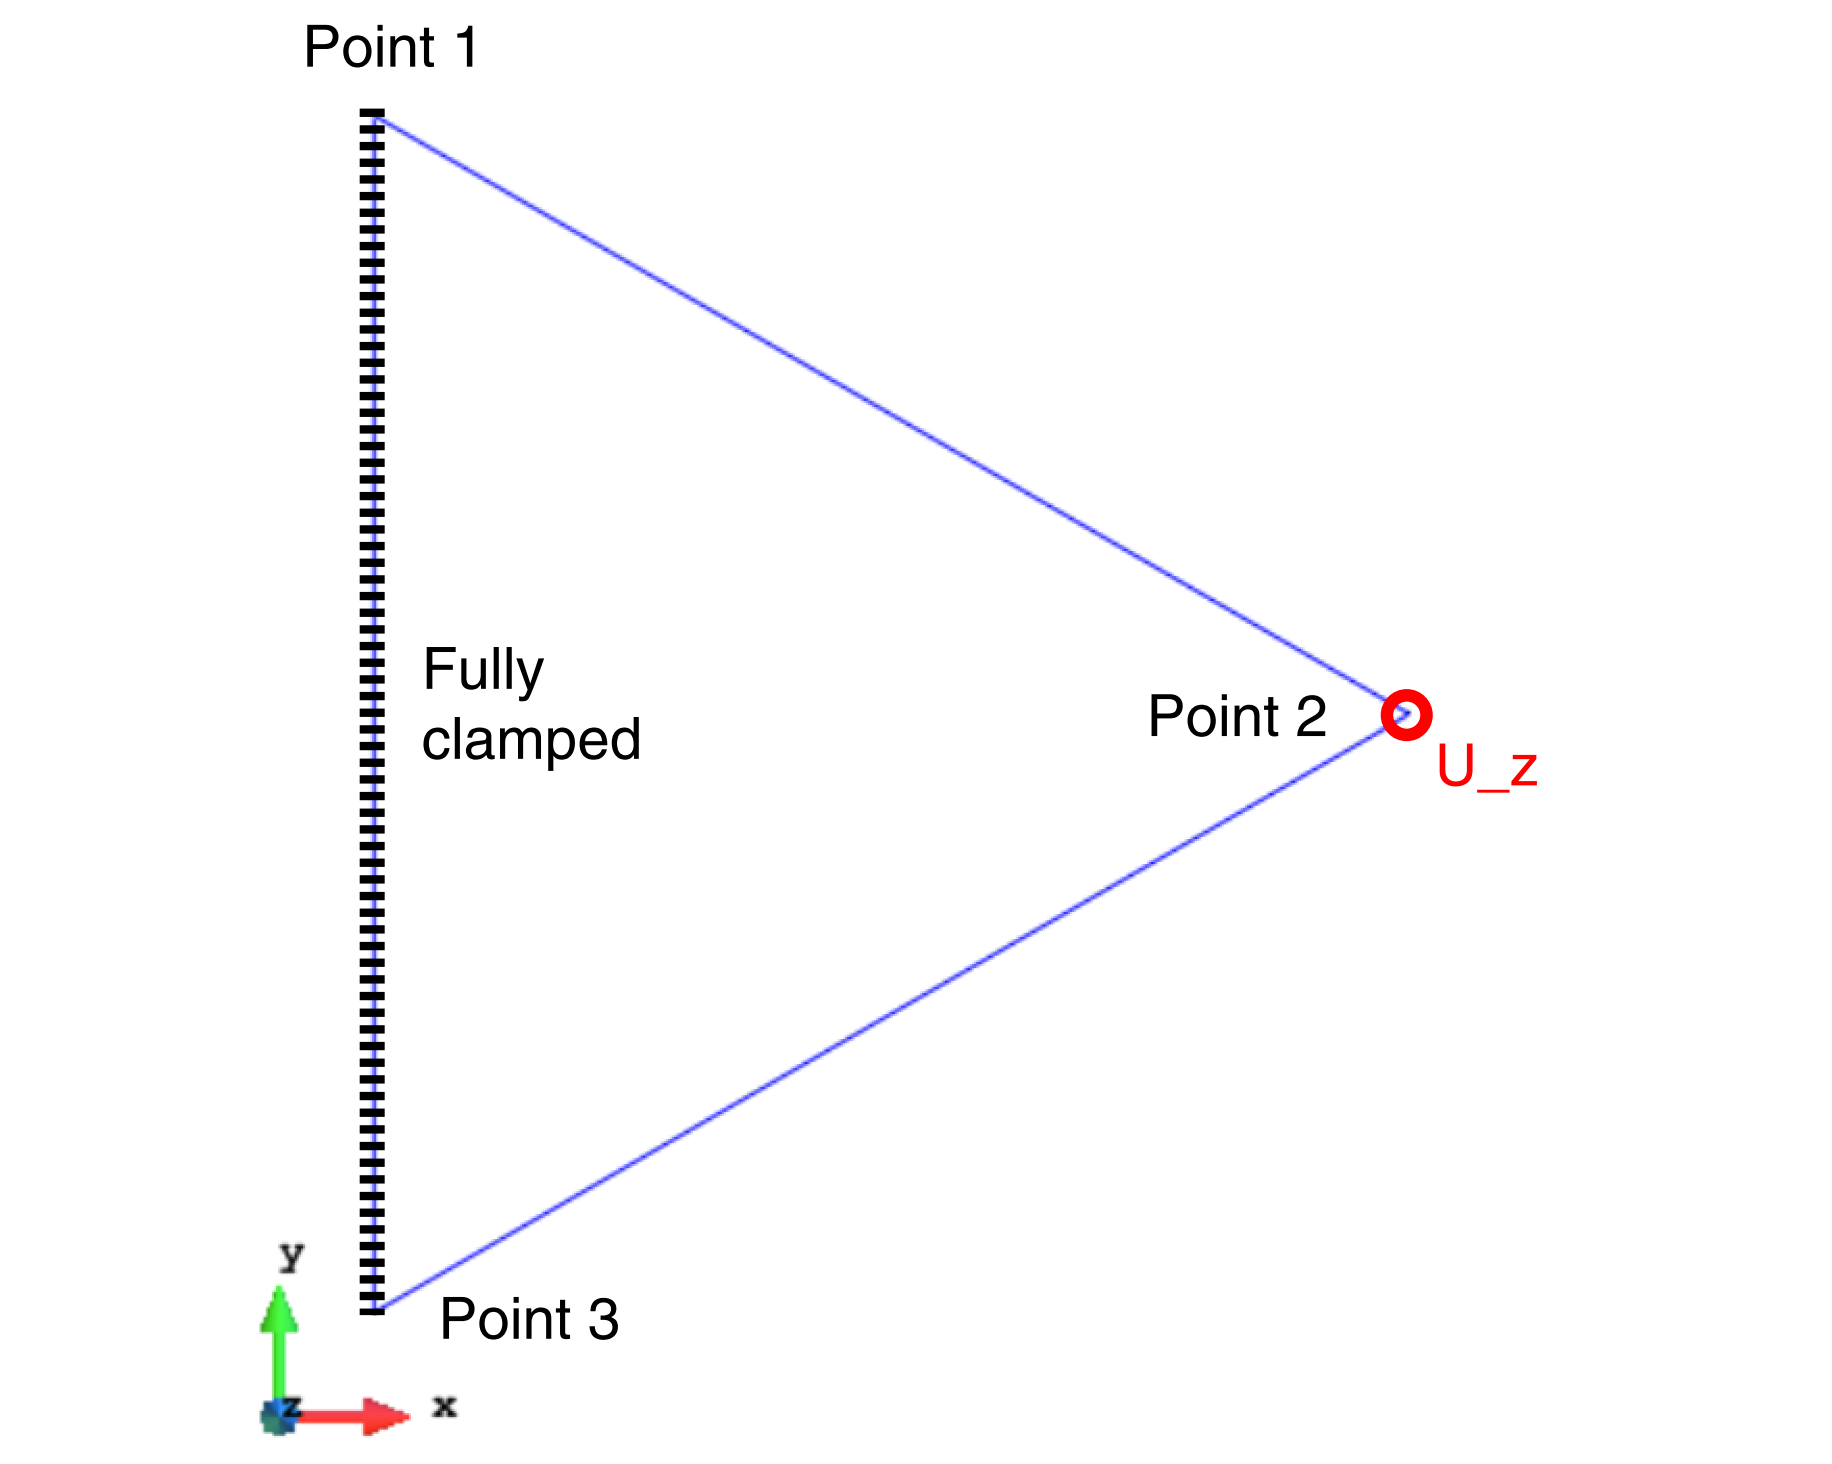
\includegraphics[width=7.3cm]
		{csdsg_single_tri_setup.png}}
	\subfloat[Displacement vs nodal ordering arrangement]
	{\label{ref_label2}
		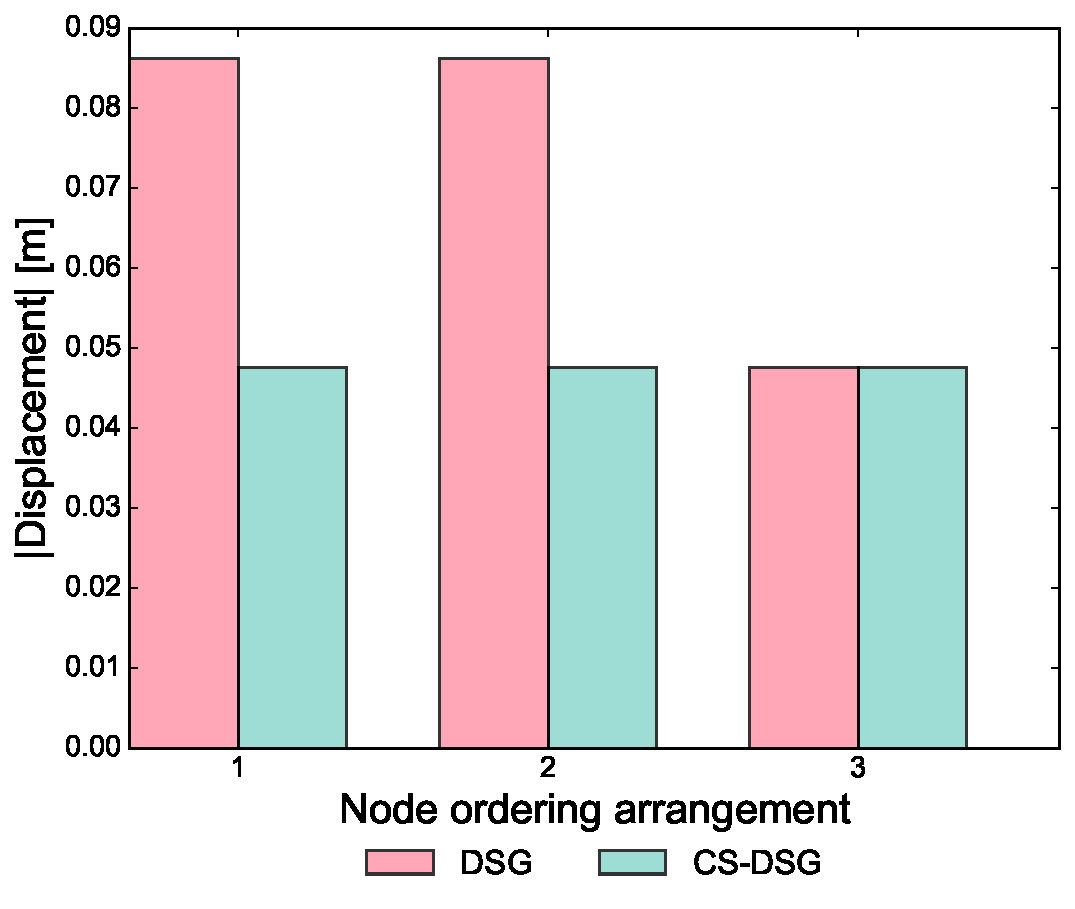
\includegraphics[width=7.3cm]
		{node_ordering_study_single_tri.pdf}}
	\caption{\label{csdsg_nodal_ordering}Sensitivity of nodal ordering between DSG and CS-DSG elements}
\end{figure}

The nodal ordering dependency of the DSG formulation is clear to see, with the third arrangement producing different displacements than the first two. Contrasting this, the CS-DSG formulation produces the exact same result across all nodal numbering arrangements, confirming it is indeed invariant of nodal numbering.

\subsection{Comparison of DSG and CS-DSG elements in the shell obstacle course}
Although the focus of the previous test was nodal numbering dependency, the accuracy of the CS-DSG has not been considered yet. The advantage of nodal numbering invariance is clearly rendered useless if the element is not accurate. Thus, the CS-DSG is run through the shell obstacle course (as per section \ref{section:shell obstacle course}) in the current section, with the original DSG formulation results presented for comparison.

\begin{figure}[H]
	\subfloat[Scorelis-Lo roof test]
	{\label{ref_label2}
		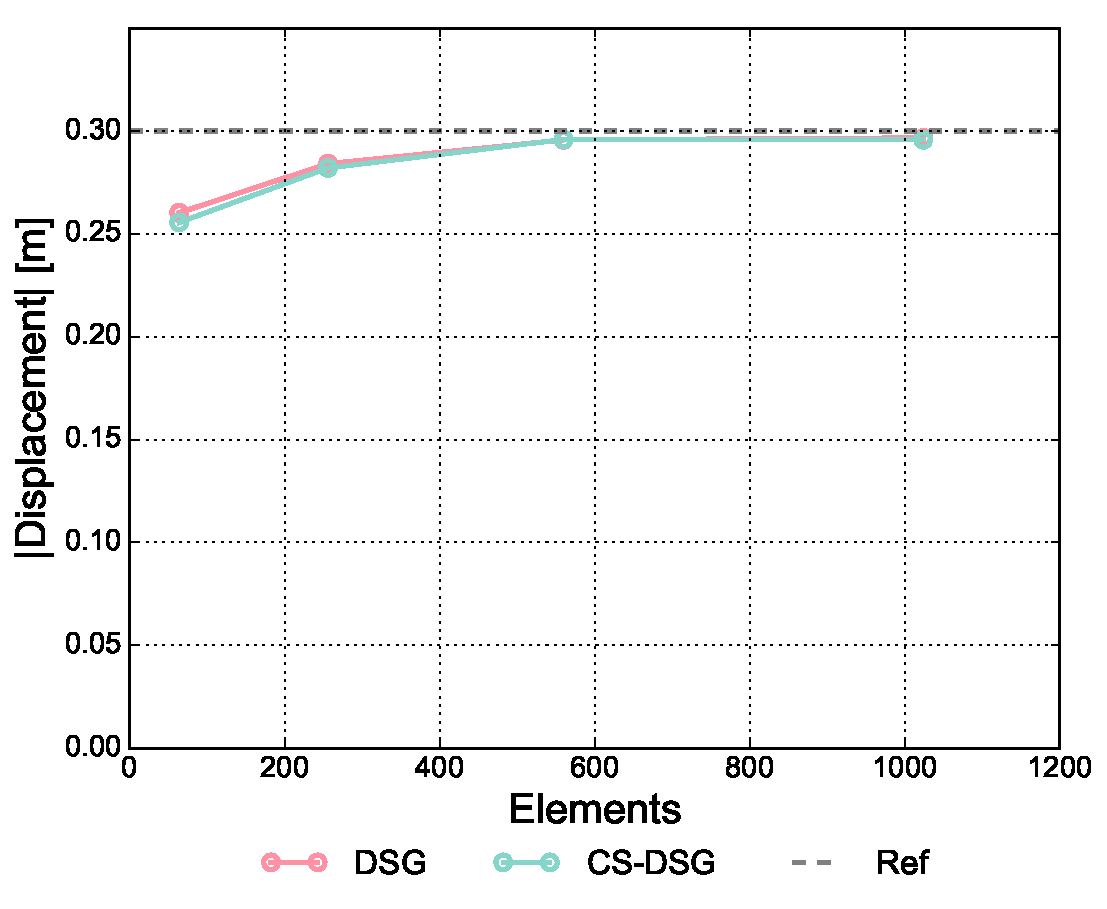
\includegraphics[width=7.3cm]
		{scordelis_structured_tri_results_csdsg.pdf}}
	\subfloat[Pinched cylinder test]
	{\label{ref_label2}
		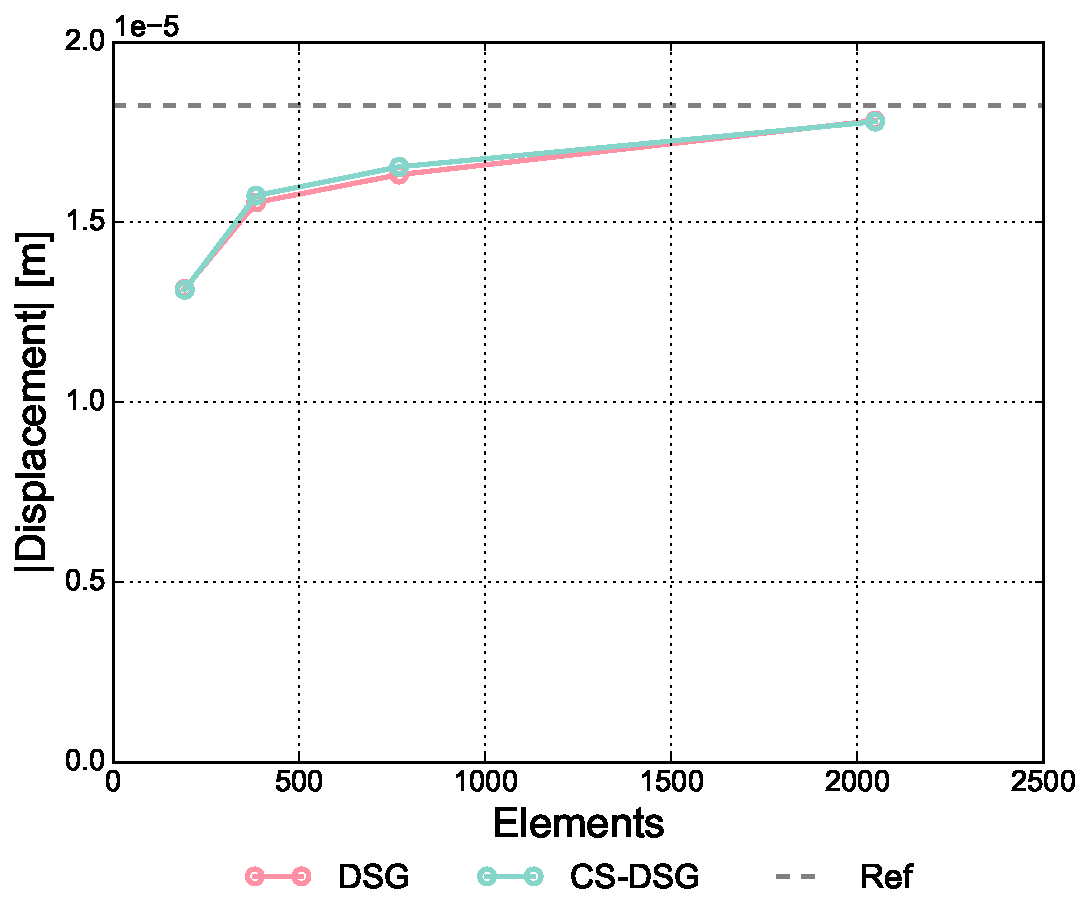
\includegraphics[width=7.3cm]
		{pinched_cyl_structured_tri_results_csdsg.pdf}}
	\\
		\subfloat[Pinched hemisphere test]
	{\label{ref_label2}
		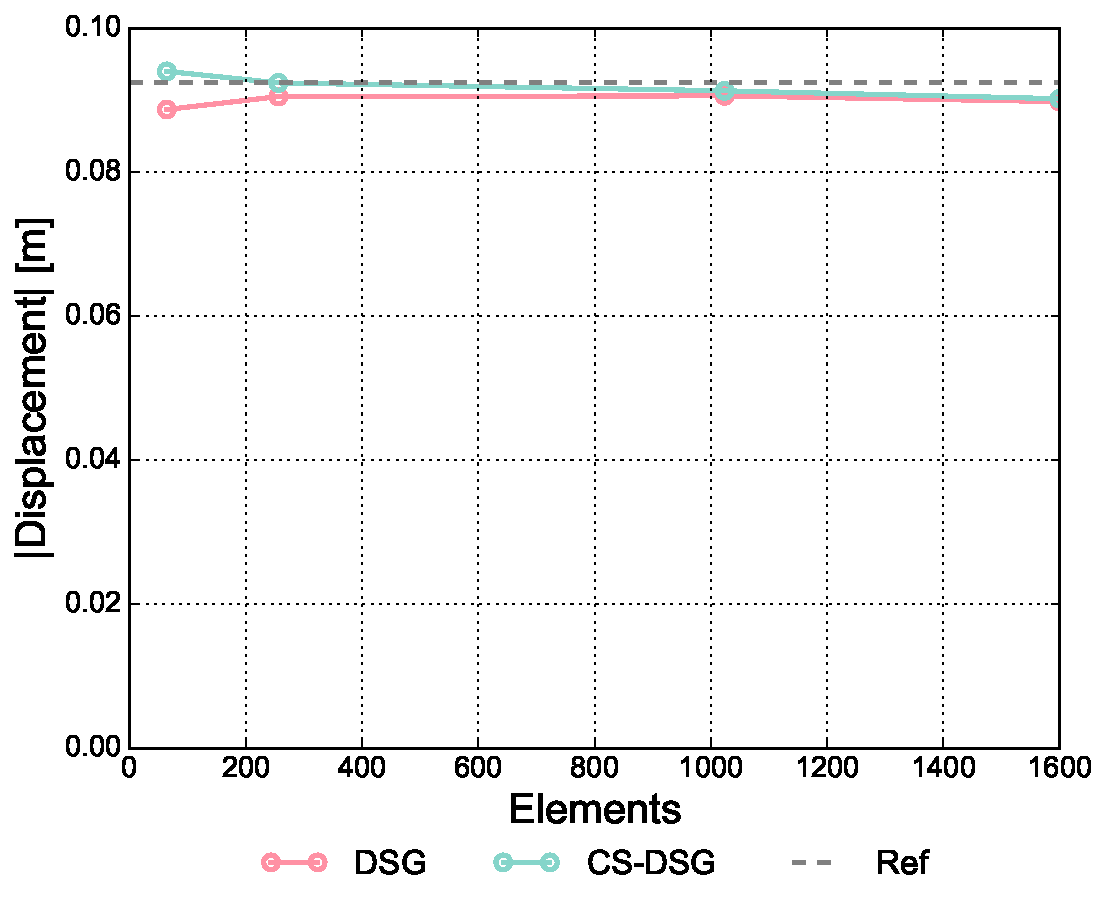
\includegraphics[width=7.3cm]
		{pinched_hemi_tri_results_CSDSG.pdf}}
	\caption{\label{csdsg_shell_obstacl}Shell obstacle course: DSG vs. CS-DSG}
\end{figure}

Results of the shell obstacle course confirm the behaviours of the DSG and CS-DSG elements converge as the mesh is refined, corresponding to the DSG nodal numbering dependency dissipating with finer meshes, as described in the original DSG formulation. The greatest difference occurring between the elements in the first data points (64 element coarse mesh) of the pinched hemisphere test is still relatively minor, highlighting that the DSG nodal dependency of this coarse mesh is already significantly diminished from that of a single triangle (refer figure \ref{csdsg_nodal_ordering} (b)). Thus, the CS-DSG element maintains the 'fine-mesh' accuracy of the original DSG element while also mitigating the nodal dependency of the original element. However, one may invoke the \textit{no free lunch} theorem, and hold the added computational effort of the CS-DSG element against the limited range of nodal dependency of the DSG element. Two questions arise to address this dichotomy: \textit{"how fast does the nodal dependency of the DSG element dissipate to negligible levels?"}, and, 
 \textit{"how gross is the additional computational effort required for the CS-DSG element?"}. 
 
\section{Appraisal of alternative DSG technology approaches}
\label{CSDSG appraisal}
In an attempt to evaluate whether the DSG or CS-DSG is more suitable for general purpose FEA use, the two questions previously posed are recalled:

\begin{itemize}
	\item \textit{"how fast does the nodal dependency of the DSG element dissipate to negligible levels?"}, and,
	\item \textit{"how gross is the additional computational effort required for the CS-DSG element?"}.
\end{itemize}

Both of these question are addressed in the subsequent sections.

\subsection{Dissipation rate of DSG nodal ordering dependency}
The dissipation rate of the DSG nodal ordering dependency is studied with the following $20\ \times\ 20\ \times\ 1$ thick square plate of isotropic material $E = 1\times10^6,\ \nu = 0.29$ subject to a uniform pressure of $P_z = -1$. Two asynchronous boundary condition cases are designed to extricate the underlying nodal numbering dependency: the first being the bottom edge fully clamped (and all others free) and the second the left edge fully clamped (and all others free). 

\begin{figure}[H]
	\subfloat[2 element mesh]
	{\label{ref_label2}
		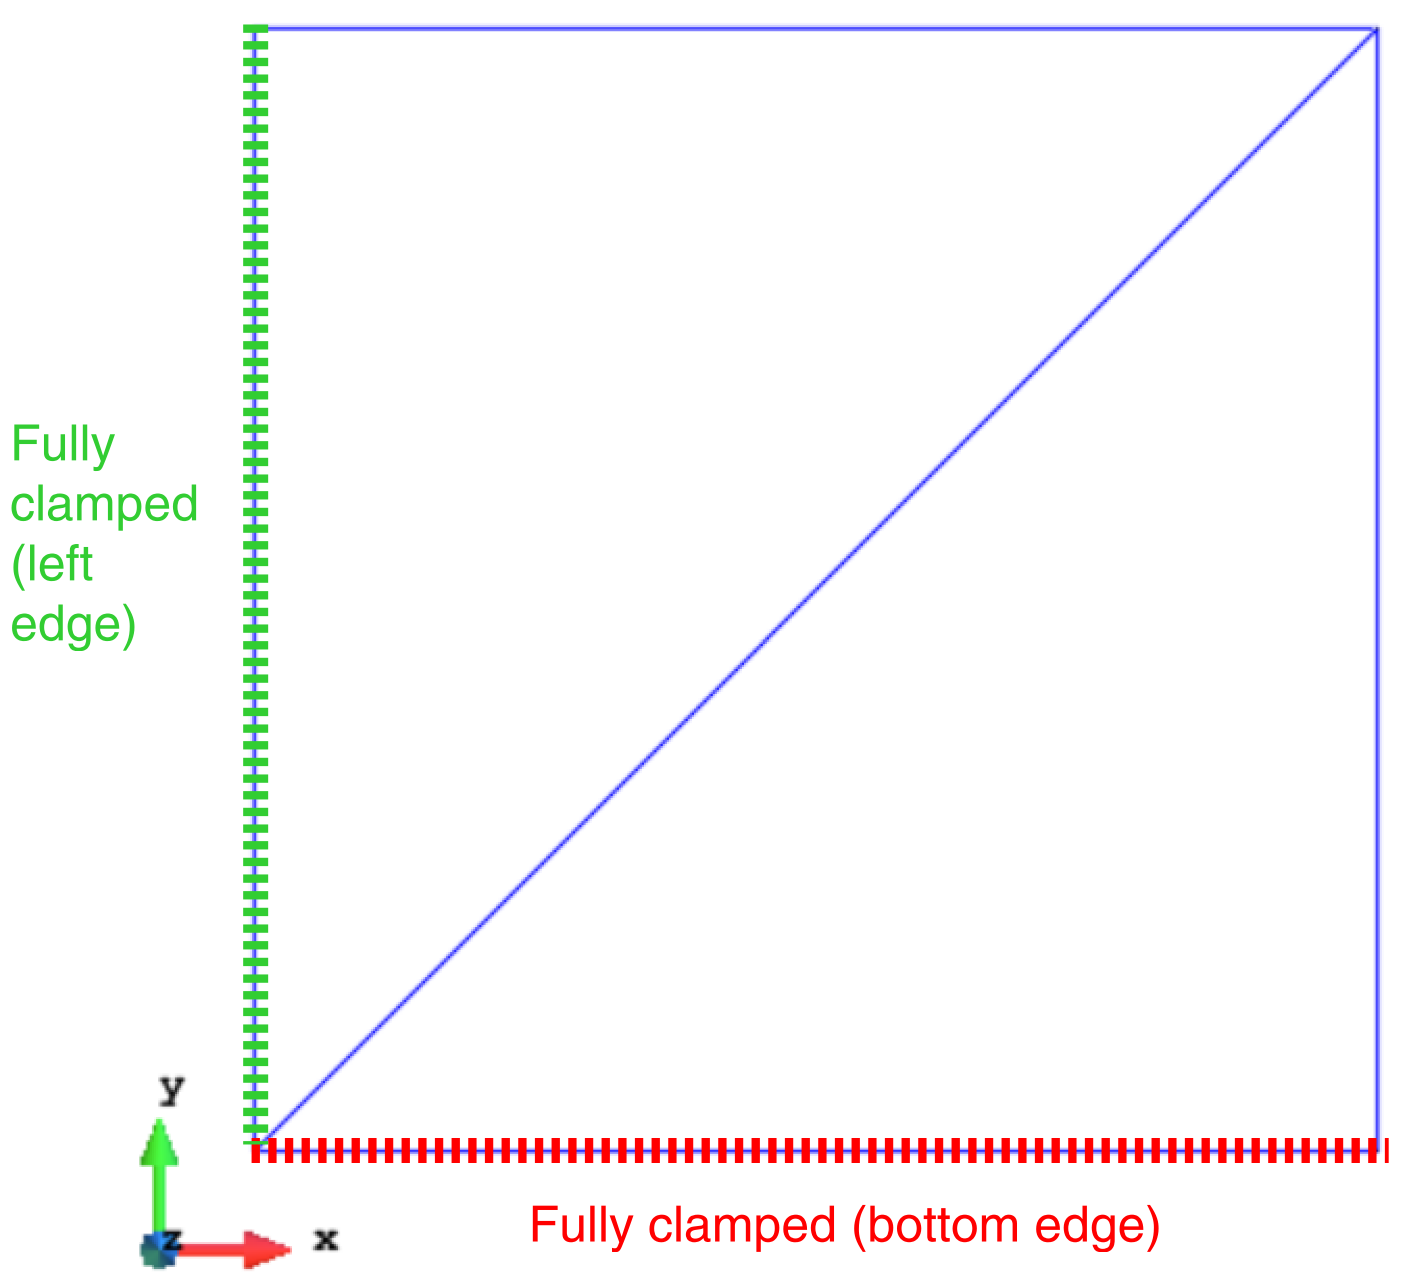
\includegraphics[width=7.3cm]
		{csdsg_nodal_dissipation_setup.png}}
	\subfloat[8 element mesh]
	{\label{ref_label2}
		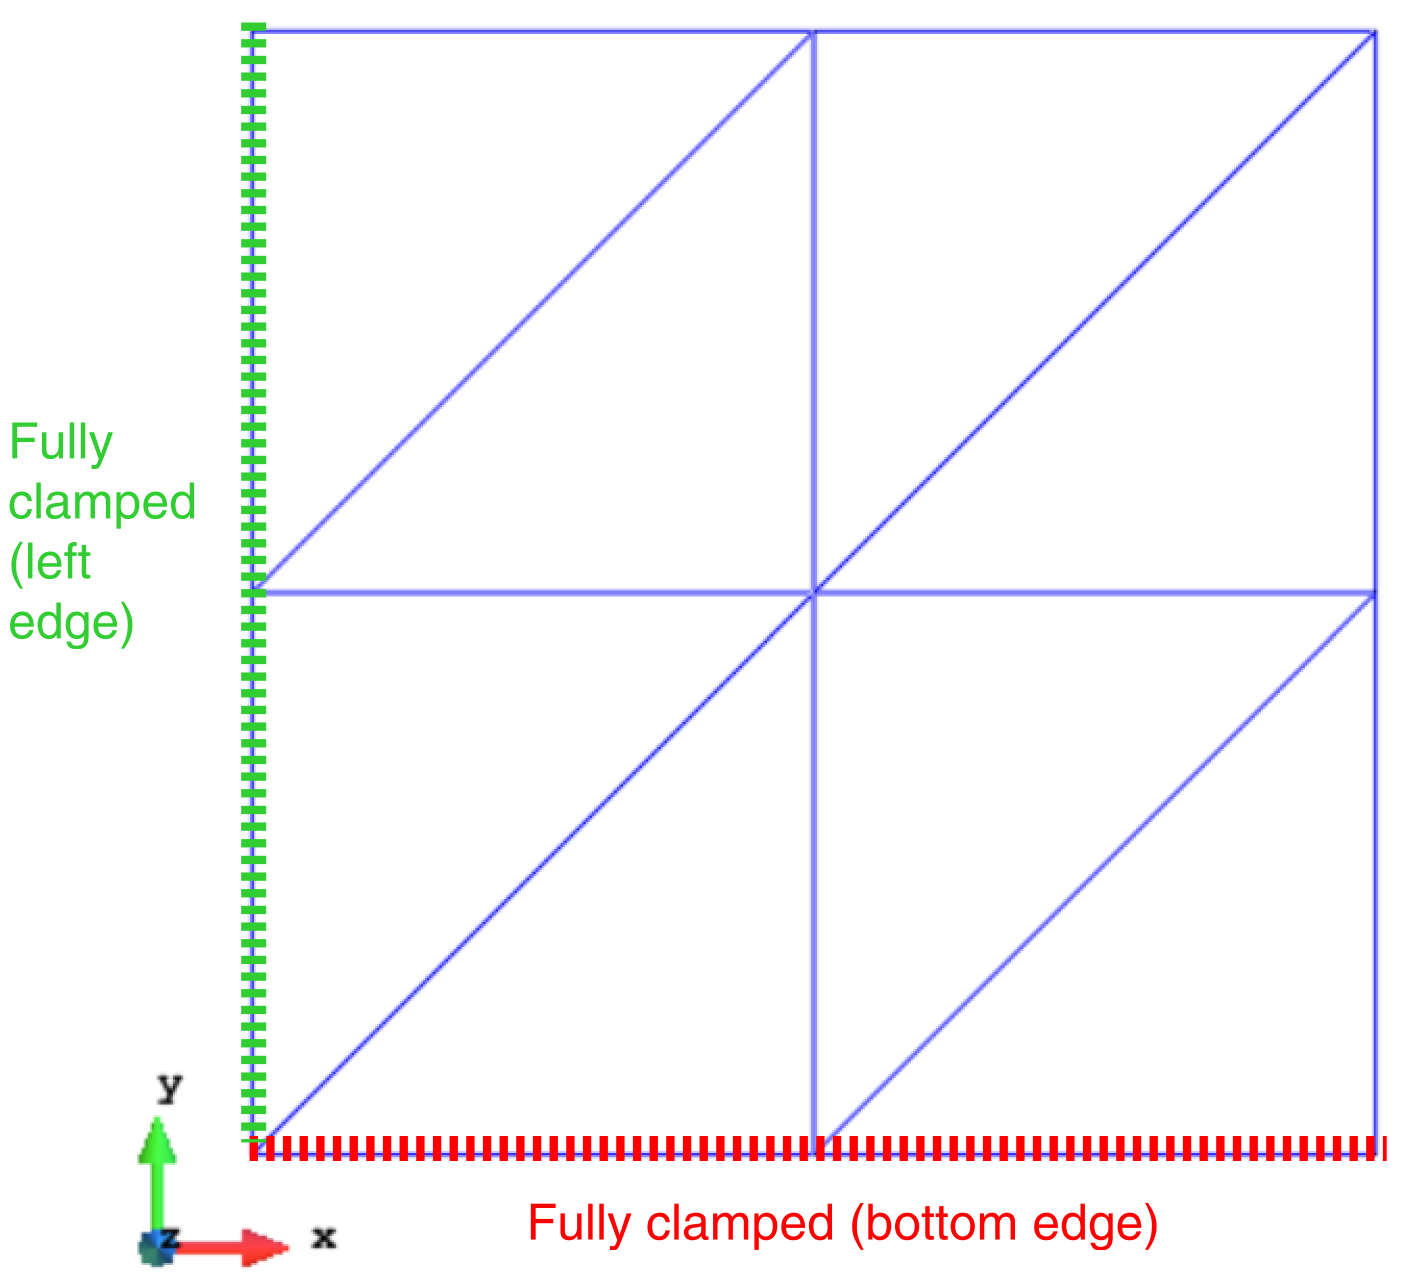
\includegraphics[width=7.3cm]
		{csdsg_nodal_dissipation_setup1.png}}
	\caption{\label{csdsg_nodal_dissipation}DSG nodal dependency dissipation rate study setup}
\end{figure}

These two boundary conditions are imposed separately, with the minimum z-displacement across the whole domain taken as the displacement of interest. The results of the study are presented below:

\begin{figure}[H]
	\centering
	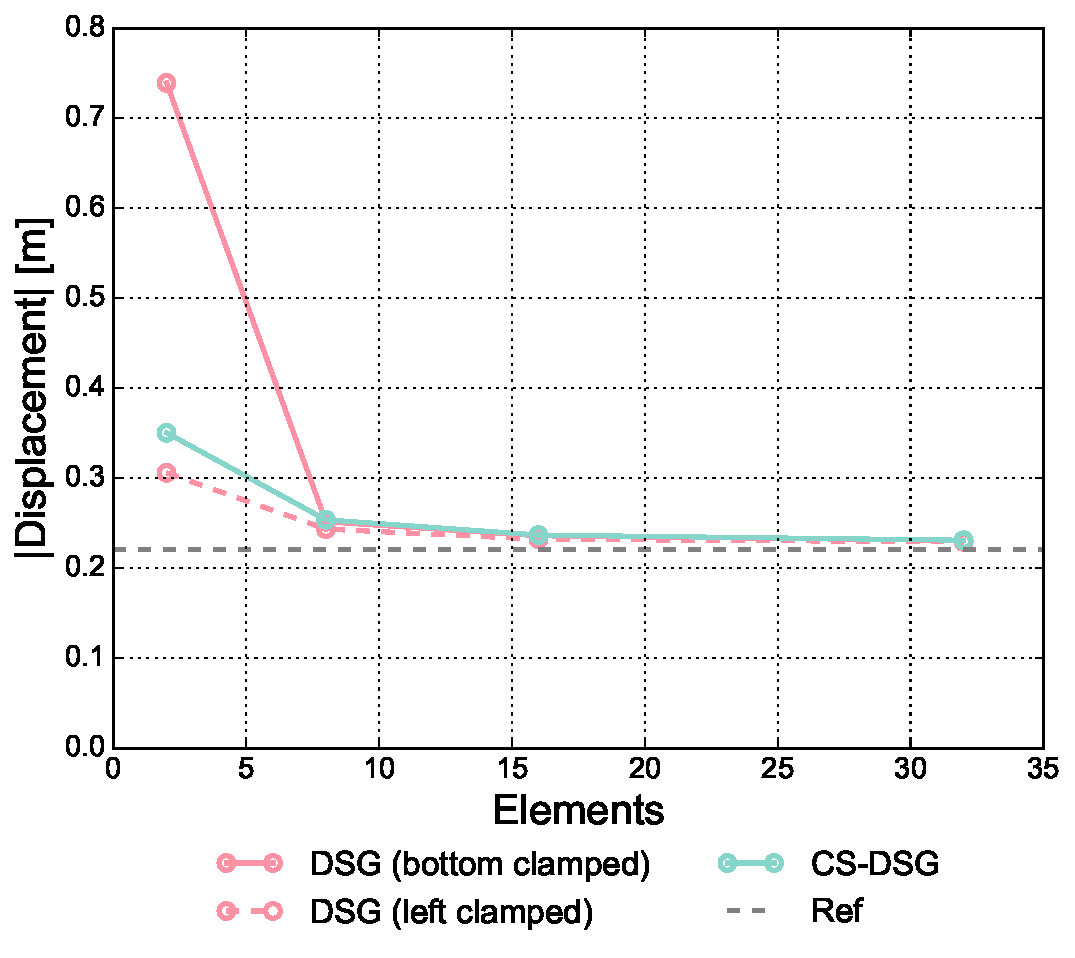
\includegraphics[width=10cm]{images/node_ordering_study.pdf}
	\caption{Nodal ordering sensitivity study of DSG formulations}
	\label{fig:Nodal ordering sensitivity study}
\end{figure}

As expected, the coarsest 2 element mesh reveals a high level of nodal numbering dependency in the DSG element, with the 2 boundary conditions producing considerably different displacement results. The CS-DSG element produced identical displacement results for this coarse mesh across both boundary conditions, as well as for all other meshes studied. The 2 element mesh also reveals that although the CS-DSG has no node-numbering dependency, this doesn't necessarily mean it is more accurate than the DSG mesh. Indeed, the left clamped DSG case is closer to the reference solution, however, the bottom clamped DSG case is quite inaccurate. It seems apparent that in this 2 element mesh, and most likely for other very coarse meshes, the CS-DSG element guarantees a result better than the worst possible DSG result but not necessarily better than the best DSG node ordering sensitive result. Despite this caveat, it's clear that the CS-DSG element produces reliably more accurate results than the DSG element for the coarsest mesh.

Progressing with mesh refinement, the 8 element mesh DSG results demonstrate almost complete convergence between the two boundary conditions, indicating negligible nodal numbering dependency. Additionally, the DSG and CS-DSG results essentially coalesce after this single level of refinement. As the mesh is refined further, differences between the 3 result cases continue to evaporate and they converge to the same reference solution of $min(u_z) = -0.22058$ calculated with an 'overkill' mesh of 11, 250 elements.

\subsection{Computational cost vs. error for DSG and CS-DSG elements}
The previous study of nodal numbering dependency confirms that although the CS-DSG element outperforms the DSG element on the coarsest meshes, the DSG nodal ordering dependency dissipates relatively quickly. Given this performance disparity, the additional computational cost associated with the CS-DSG element must be known to make an informed decision as to what element should be preferred for general use. 

Since the shear B-matrix is the only point of difference between the two formulations, the computational cost discrepancy can be reduced to the time taken to construct the shear B-matrix for each element. The previous analysis' 32 element case was re-run with the average wall time for the construction of the shear B-matrix of the DSG element determined to be 12.000 ns while the CS-DSG counterpart was 13.438 ns. As expected, the simpler DSG formulation is quicker than the CS-DSG formulation, with the latter taking 12\% longer than the former to construct. If the results of the previous analysis are converted to cumulative element shear B-matrix construction time ($= elements \times average\ time\ to\ construct\ shear\ B\ matrix$, i.e. the time taken per job run to construct all shear B-matrices) vs. percentage error (against the reference value) the following graph is produced:

\begin{figure}[H]
	\centering
	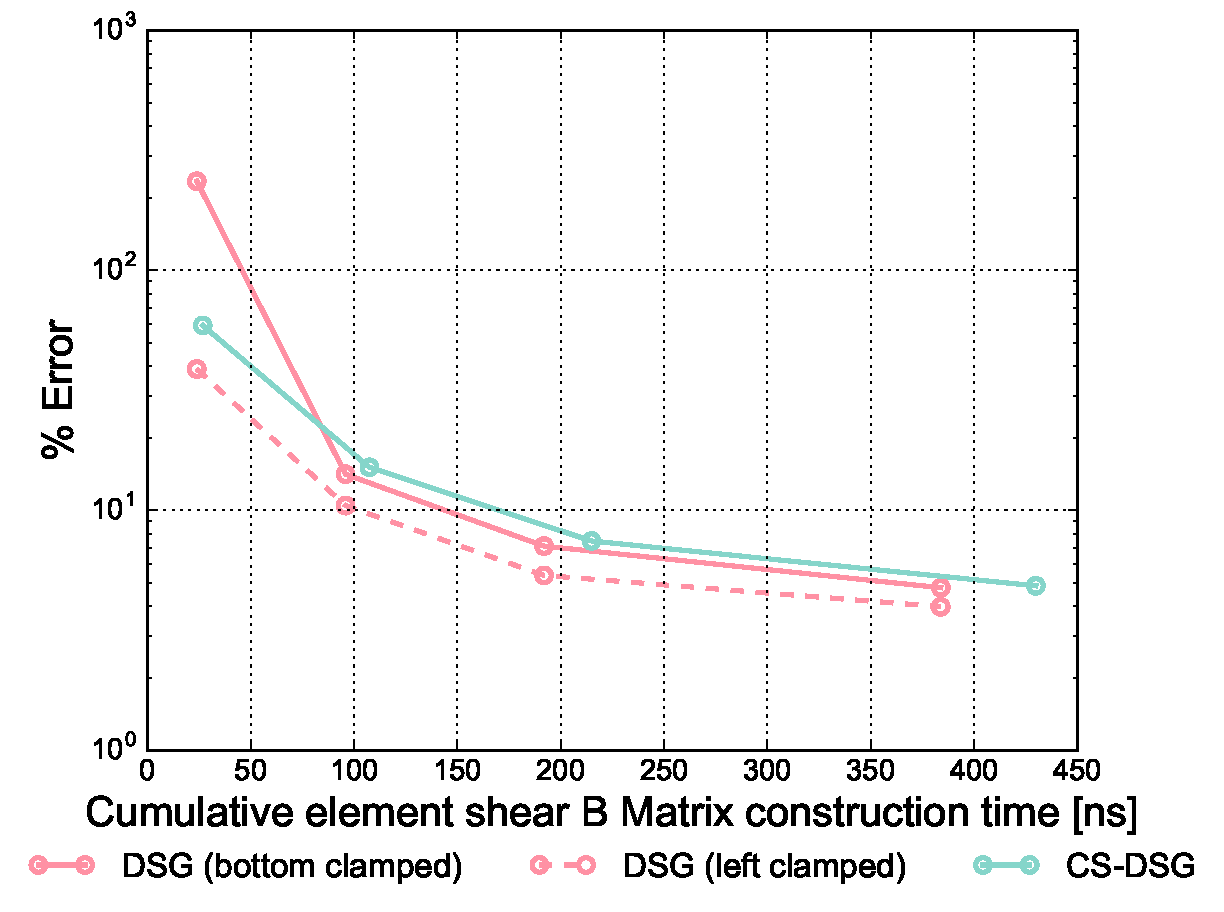
\includegraphics[width=10cm]{images/node_ordering_study_error.pdf}
	\caption{Computational cost vs \% error of DSG formulations}
	\label{fig:Computational cost vs error of DSG formulations}
\end{figure}

Practical FEA is often driven by the tension of obtaining accurate results in a timely manner, with minor differences in element speeds magnified into substantial time delays when a large number of iterations are necessary (such as fine dynamic analysis and highly non-linear analysis). The above graph highlights that the DSG element actually reaches a lower percentage error level 'before' (in the sense of time) the CS-DSG element for all meshes except the first. That is, for typical practical meshes (indeed 2 element meshes, especially linear triangles, are ill-advised in practise), the DSG element offers comparable accuracy to the CS-DSG element at a lower computational cost. Exceptional cases will no doubt arise where the CS-DSG element is more suitable, a possible example being the analysis of an I-beam where flange meshes are often naturally coarse due to the size difference between the flanges and the web, however this merely reinforces the importance of correct structural modelling of the system at hand and knowledge concerning the interplay of assumptions, element choices and potential deleterious consequences: a central theme of this thesis.

\section{Chapter summary}
Despite the DSG element technology significantly improving the pure displacement-based constant strain triangle, it possesses artificially introduced nodal numbering dependency. The DSGc3 proof of concept parametric unit triangle formulation developed by Prof. Bletzinger effectively addresses this but is yet to be extended to general skew Cartesian triangles. Another approach, the CS-DSG element, has been implemented in Kratos and eliminates the nodal numbering dependency apparent in coarse meshes while converging to the original DSG results in the fine mesh limit. A study of the dissipation rate of DSG nodal ordering dependency against the additional cost of mitigating it with the CS-DSG was presented. In light of the DSG nodal ordering dependency diminishing quickly, the DSG element appears to be the preferred element for general analysis, while fringe cases involving very coarse meshes would benefit from employing the CS-DSG element.